% SC4064 --- Chapter 3: GPU Memory: Global, Shared, Constant, Coalescing and Bank Conflicts (0->100)
\chapter{GPU Memory: Global, Shared, Constant, Coalescing and Bank Conflicts}
\label{ch:memory}
\sloppy

\begin{quote}
\emph{``Flops are cheap, data movement is expensive.''} A GPU can do thousands of multiplies per nanosecond but waits hundreds of cycles for one uncoalesced DRAM access. Understanding where data lives and how warps fetch it is the difference between 10\% and 90\% of peak bandwidth.
\end{quote}

\noindent\fbox{\parbox{\dimexpr\linewidth-2\fboxsep-2\fboxrule}{%
\textbf{From zero: no GPU memory background assumed.} We start from the idea that memory is a hierarchy---registers, caches, DRAM---and build the GPU version: global (big, slow), shared (tiny, fast, programmer-managed), constant (broadcast), plus the two performance laws that govern them: coalescing for global and bank conflicts for shared.}}
\vspace{0.4em}

\section*{Learning Outcomes}
After this chapter you will be able to:
\begin{enumerate}[label=(L\arabic*)]
    \item name the GPU memory spaces, their sizes, lifetimes and who manages them;
    \item explain coalesced versus strided global access and quantify the bandwidth impact;
    \item describe shared-memory banks, why conflicts serialise, and how to pad or permute to avoid them;
    \item choose appropriate memory (global, shared, constant, registers) for a given access pattern;
    \item apply tiling with \texttt{\_\_syncthreads()} to exploit shared memory correctly.
\end{enumerate}

% ============================================================
\section{The GPU Memory Hierarchy}
\label{sec:mem-hierarchy}
\paragraph{Intuition.} Think of a building site. Registers are tools in your hands (1 cycle, private to a thread). Shared memory is the workbench on your floor (20--30 cycles, shared by a block, you control). L1/L2 are the site store (80--200 cycles, hardware-managed). Global memory (HBM/DRAM) is the warehouse across town (300--500 cycles, visible to all). Constant memory is a loudspeaker: one value broadcast to every thread efficiently when all read the same address.

\begin{table}[h]\centering\small
\begin{tabular}{lcccc}
\toprule
Space & Size & Latency & Scope & Managed by\\
\midrule
Registers & 64K $\times$ 32-bit / SM & 1 & thread-private & compiler\\
Shared (scratchpad) & 48--164\,KiB / SM & 20--30 & block & programmer\\
L1 / L2 cache & 128\,KiB / SM, 40--50\,MiB dev. & 30 / 200 & SM / device & hardware\\
Global (HBM) & 16--80\,GiB & 300--500 & device + host & programmer\\
Constant & 64\,KiB & 5 (hit) & device (broadcast) & programmer\\
\bottomrule
\end{tabular}
\caption{GPU memory spaces at a glance. Latencies are approximate (Ampere/Hopper). Shared and registers are the only spaces where you control placement explicitly.}
\end{table}

\begin{definition}[Global, shared, constant]
\emph{Global} memory is large off-chip DRAM, allocated with \texttt{cudaMalloc}, visible to all threads and the host. \emph{Shared} memory (\texttt{\_\_shared\_\_}) is on-chip SRAM partitioned per SM, visible only within a block, lifetime = block, explicit barrier needed. \emph{Constant} memory (\texttt{\_\_constant\_\_}) is read-only, cached, optimised for uniform reads where all threads in a warp read the same address simultaneously.
\end{definition}

\begin{figure}[h]\centering
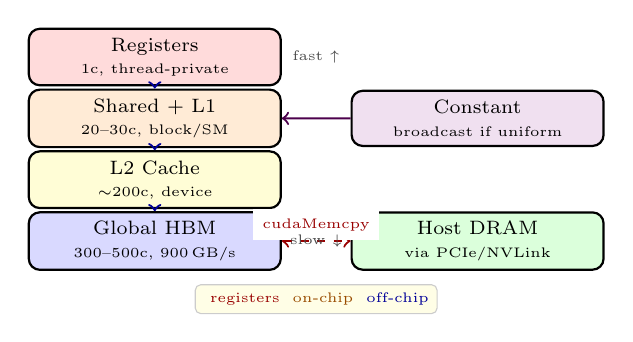
\begin{tikzpicture}[scale=0.82, every node/.style={font=\scriptsize},
  lev/.style={draw, thick, rounded corners=4pt, align=center, minimum height=0.70cm}]
\node[lev, fill=red!14, minimum width=3.2cm] (reg) at (0,2.7) {Registers\\{\tiny 1c, thread-private}};
\node[lev, fill=orange!16, minimum width=3.2cm] (sh) at (0,1.75) {Shared + L1\\{\tiny 20--30c, block/SM}};
\node[lev, fill=yellow!16, minimum width=3.2cm] (l2) at (0,0.80) {L2 Cache\\{\tiny $\sim$200c, device}};
\node[lev, fill=blue!15, minimum width=3.2cm] (gl) at (0,-0.15) {Global HBM\\{\tiny 300--500c, 900\,GB/s}};
\node[lev, fill=violet!12, minimum width=3.2cm] (co) at (5.0,1.75) {Constant\\{\tiny broadcast if uniform}};
\node[lev, fill=green!14, minimum width=3.2cm] (dr) at (5.0,-0.15) {Host DRAM\\{\tiny via PCIe/NVLink}};
\draw[->, thick, blue!60!black] (reg) -- (sh);
\draw[->, thick, blue!60!black] (sh) -- (l2);
\draw[->, thick, blue!60!black] (l2) -- (gl);
\draw[<->, thick, red!60!black, dashed] (gl) -- (dr) node[midway, above, font=\tiny, fill=white] {cudaMemcpy};
\draw[->, thick, violet!60!black] (co) -- (sh);
\node[font=\tiny, text=gray!60!black, align=center] at (2.5,2.7) {fast $\uparrow$};
\node[font=\tiny, text=gray!60!black, align=center] at (2.5,-0.15) {slow $\downarrow$};
\node[font=\tiny, align=left, fill=yellow!10, draw=gray!40, rounded corners=2pt, inner sep=3pt] at (2.5,-1.05) {\textcolor{red!60!black}{$\blacksquare$ registers} \textcolor{orange!60!black}{$\blacksquare$ on-chip} \textcolor{blue!60!black}{$\blacksquare$ off-chip}};
\end{tikzpicture}
\caption{GPU memory hierarchy: small fast memories at the top (registers, shared/L1), large slow HBM at the bottom. Constant broadcasts; host link is the narrowest pipe.}
\label{fig:mem-hierarchy}
\end{figure}

% ============================================================
\section{Global Memory and Coalescing}
\label{sec:coalescing}
Global accesses move in 32-, 64- or 128-byte \emph{sectors} (cache lines). When 32 threads of a warp access contiguous 4-byte floats at \texttt{base + tid*4}, the hardware coalesces them into one or two sectors---full bandwidth. When they access strided (\texttt{base + tid*32*4}) or random addresses, the same 32 requests scatter across 32 sectors---you fetch 32$\times$ more bytes than needed and waste 97\% of bandwidth.

\begin{figure}[h]\centering
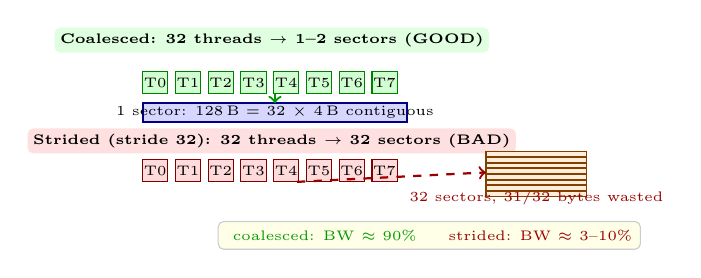
\begin{tikzpicture}[scale=0.80, every node/.style={font=\scriptsize}]
% Coalesced
\node[font=\tiny\bfseries, fill=green!12, rounded corners=2pt, inner sep=2pt] at (2.2,2.55) {Coalesced: 32 threads $\to$ 1--2 sectors (GOOD)};
\foreach \i in {0,...,7} {
  \draw[fill=green!18, draw=green!50!black] (0.15+\i*0.52,1.70) rectangle (0.55+\i*0.52,2.05);
  \node[font=\tiny] at (0.35+\i*0.52,1.875) {T\i};
}
\draw[fill=blue!16, draw=blue!50!black, thick] (0.15,1.25) rectangle (4.35,1.55);
\node[font=\tiny] at (2.25,1.40) {1 sector: 128\,B = 32 $\times$ 4\,B contiguous};
\draw[->, thick, green!60!black] (2.25,1.70) -- (2.25,1.55);
% Strided
\node[font=\tiny\bfseries, fill=red!12, rounded corners=2pt, inner sep=2pt] at (2.2,0.95) {Strided (stride 32): 32 threads $\to$ 32 sectors (BAD)};
\foreach \i in {0,...,7} {
  \draw[fill=red!14, draw=red!50!black] (0.15+\i*0.52,0.30) rectangle (0.55+\i*0.52,0.65);
  \node[font=\tiny] at (0.35+\i*0.52,0.475) {T\i};
  \draw[fill=orange!14, draw=orange!50!black] (5.6,0.70-\i*0.09) rectangle (7.2,0.78-\i*0.09);
}
\node[font=\tiny, text=red!60!black] at (6.4,0.05) {32 sectors, 31/32 bytes wasted};
\draw[->, thick, red!60!black, dashed] (2.6,0.30) -- (5.6,0.45);
% Right side annotation
\node[font=\tiny, align=left, fill=yellow!10, draw=gray!40, rounded corners=2pt, inner sep=3pt] at (4.7,-0.55) {\textcolor{green!60!black}{$\blacksquare$ coalesced: BW $\approx$ 90\%} \quad \textcolor{red!60!black}{$\blacksquare$ strided: BW $\approx$ 3--10\%}};
\end{tikzpicture}
\caption{Coalescing: contiguous warp accesses collapse to one transaction; strided/random accesses explode to many. Structure-of-arrays and transposed layouts exist to restore coalescing.}
\label{fig:coalescing}
\end{figure}

The fix is usually a data layout change. Array-of-structures (AoS) \texttt{\{x,y,z\}} per thread is strided when threads read only \texttt{x}; structure-of-arrays (SoA) \texttt{x[], y[], z[]} is coalesced. Transposing a matrix before a column-wise kernel has the same effect. Unified Memory (\texttt{cudaMallocManaged}) hides the copy but not the coalescing cost---the access pattern still governs performance.

\begin{example}[SoA vs.\ AoS]
100K particles with \texttt{struct \{float x,y,z;\} p[N];} and kernel \texttt{p[tid].x += 1;} is strided (stride 12\,B). Rewriting as \texttt{float x[N],y[N],z[N];} and \texttt{x[tid]+=1;} is contiguous and typically $4$--$8\times$ faster despite identical maths.
\end{example}

% ============================================================
\section{Shared Memory and Bank Conflicts}
\label{sec:shared-banks}
Shared memory is split into 32 \emph{banks}, each 4 bytes wide, with successive 4-byte words in successive banks (round-robin). If 32 threads of a warp access 32 different banks, all serve in one cycle. If two or more threads hit the same bank with different addresses (a \emph{bank conflict}), accesses serialise---$k$-way conflict costs $k$ cycles. Broadcast (all threads read the same address) is free.

\begin{figure}[h]\centering
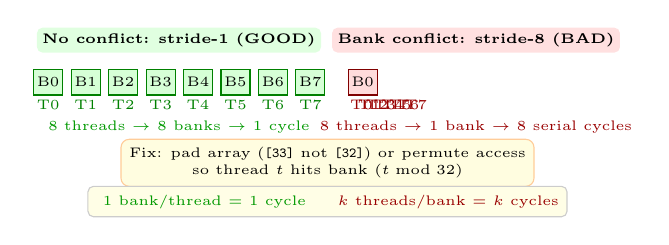
\begin{tikzpicture}[scale=0.82, every node/.style={font=\scriptsize}]
% No conflict
\node[font=\tiny\bfseries, fill=green!12, rounded corners=2pt, inner sep=2pt] at (2.4,2.55) {No conflict: stride-1 (GOOD)};
\foreach \b in {0,...,7} {
  \draw[fill=green!16, draw=green!50!black] (0.15+\b*0.58,1.70) rectangle (0.60+\b*0.58,2.10);
  \node[font=\tiny] at (0.375+\b*0.58,1.90) {B\b};
  \node[font=\tiny, text=green!50!black] at (0.375+\b*0.58,1.55) {T\b};
}
\node[font=\tiny, text=green!60!black] at (2.4,1.20) {8 threads $\to$ 8 banks $\to$ 1 cycle};
% Conflict
\node[font=\tiny\bfseries, fill=red!12, rounded corners=2pt, inner sep=2pt] at (7.0,2.55) {Bank conflict: stride-8 (BAD)};
\foreach \b in {0,...,7} {
  \draw[fill=red!14, draw=red!50!black] (5.0+0.02,1.70) rectangle (5.45+0.02,2.10);
  \node[font=\tiny] at (5.225+0.02,1.90) {B0};
  \node[font=\tiny, text=red!60!black] at (5.225+\b*0.12,1.55) {T\b};
}
\node[font=\tiny, text=red!60!black, align=center] at (7.0,1.20) {8 threads $\to$ 1 bank $\to$ 8 serial cycles};
% Padding fix annotation
\node[font=\tiny, align=center, fill=yellow!12, draw=orange!40, rounded corners=3pt, inner sep=3pt] at (4.7,0.65) {Fix: pad array (\texttt{[33]} not \texttt{[32]}) or permute access\\so thread $t$ hits bank $(t\bmod 32)$};
\node[font=\tiny, align=left, fill=yellow!10, draw=gray!40, rounded corners=2pt, inner sep=3pt] at (4.7,0.05) {\textcolor{green!60!black}{$\blacksquare$ 1 bank/thread = 1 cycle} \quad \textcolor{red!60!black}{$\blacksquare$ $k$ threads/bank = $k$ cycles}};
\end{tikzpicture}
\caption{Shared-memory banks: contiguous access hits distinct banks (fast); power-of-two strides collapse onto one bank (conflict). Padding breaks the stride.}
\label{fig:bank-conflict}
\end{figure}

Classic fix: for a tile \texttt{float tile[32][32]}, column access \texttt{tile[threadIdx.x][*]} has stride 32 and conflicts; declare \texttt{tile[32][33]} to skew banks so each row starts one bank offset. Alternatively, have warps cooperatively load in coalesced/shared-friendly order, \texttt{\_\_syncthreads()}, then compute.

\paragraph{Constant and unified memory.} Constant memory shines when a warp reads one address together: the single value is fetched once and broadcast, not 32 separate loads. Mark read-only tables bigger than 64\,KiB with \texttt{\_\_restrict\_\_ const} and let the L1 handle them. Unified Memory (\texttt{cudaMallocManaged}) gives a single pointer for host and device and migrates pages on demand---convenient for prototyping and oversubscription, but the same coalescing and bank rules apply after migration. Prefetch with \texttt{cudaMemPrefetchAsync} and advise with \texttt{cudaMemAdvise} to avoid page-fault storms.

\begin{remark}[Quick checklist before you optimise]
(1) Is global access coalesced? Check with Nsight Compute's ``Memory Chart'' or count sectors per warp. (2) Is shared access bank-conflict-free? Nsight's ``Shared Memory'' counter shows conflict rate. (3) Are you using the right space? A common mistake is putting a broadcast table in global instead of constant, or spilling registers to local memory by using too many per thread---both visible in \texttt{ptxas} spill reports (\texttt{-Xptxas -v}).
\end{remark}

\begin{lstlisting}[language=C++, caption={Coalesced vs.\ strided global access: same work, very different bandwidth.}, label={lst:coalescing}]
__global__ void coalesced(float *a, float *b, int n){
    int tid = blockIdx.x*blockDim.x + threadIdx.x;
    if(tid<n) b[tid] = a[tid];               // contiguous: 1 sector/warp
}
__global__ void strided(float *a, float *b, int n, int stride){
    int tid = blockIdx.x*blockDim.x + threadIdx.x;
    if(tid<n) b[tid*stride] = a[tid*stride]; // stride*4 bytes apart: many sectors
}
// Measure: coalesced ~700 GB/s, strided(32) ~20 GB/s on same GPU.
\end{lstlisting}

\begin{lstlisting}[language=C++, caption={Shared-memory tiling for 1-D stencil: coalesced load, no bank conflicts, barrier.}, label={lst:shared-tile}]
__global__ void stencil1D(float *in, float *out, int n){
    __shared__ float tile[256+2]; // block + halo (padding avoids conflict when needed)
    int tid = blockIdx.x*blockDim.x + threadIdx.x;
    int lid = threadIdx.x;
    // coalesced global -> shared
    tile[lid+1] = (tid<n) ? in[tid] : 0;
    if(lid==0) tile[0] = (tid>0) ? in[tid-1] : 0;
    if(lid==blockDim.x-1) tile[lid+2] = (tid+1<n) ? in[tid+1] : 0;
    __syncthreads(); // all loads done before compute
    if(tid<n) out[tid] = 0.25f*tile[lid] + 0.5f*tile[lid+1] + 0.25f*tile[lid+2];
    // no __syncthreads needed after: no cross-thread reuse
}
\end{lstlisting}

\begin{example}[End-to-end: matrix transpose with and without shared tiling]
Naive transpose \texttt{out[j*W+i]=in[i*H+j]} is coalesced on read but strided on write (or vice versa). A tiled version loads a $32\times32$ tile into shared with coalesced reads, \texttt{\_\_syncthreads()}, then writes transposed from shared to global---both sides coalesced and bank-conflict-free with padding $[32][33]$. The tiled kernel is typically $3$--$7\times$ faster on large matrices, a textbook win from two ideas in this chapter composed together.
\end{example}

\begin{remark}[Nsight check]
Profile the transpose pair with \texttt{ncu --metrics l1tex\_\_t\_sectors\_pipe\_lsu\_mem\_global\_op\_ld.sum,l1tex\_\_t\_sectors\_pipe\_lsu\_mem\_global\_op\_st.sum}. The naive shows $\sim$32$\times$ sectors per warp on one side; the tiled shows $\sim$1--2 on both. The ratio matches your wall-clock speedup---when counters and clocks agree, you understand the bottleneck.
\end{remark}

\paragraph{Takeaway.} Global optimisation is about addresses: make warps contiguous. Shared optimisation is about banks: make threads hit distinct banks. Both are layout problems, not maths problems---you often fix them by transposing data or padding an array, not by changing FLOPs.

\smallskip

% memory chapter checkpoint: coalescing + banks mastered
% ============================================================
\section{Exercises}
\label{sec:ch03-exercises}
\begin{enumerate}[label=E3.\arabic*, leftmargin=*, itemsep=0.6em]
    \item \textbf{Memory choice.} For each pattern, pick the best space (registers, shared, constant, global) and justify: (a) per-thread private accumulator, (b) 64 floats reused by all threads in a block 10 times, (c) a 4\,KiB lookup table where every thread in a warp reads the same entry, (d) a 100\,MiB input streamed once.
    \item \textbf{Coalescing arithmetic.} A warp reads 4-byte floats. Contiguous needs 1 $\times$ 128\,B sector. Stride-8 needs how many sectors? If peak is 900\,GB/s, estimate attained BW for each. How does SoA rescue AoS here?
    \item \textbf{Bank conflict.} Shared memory has 32 banks. A kernel has 32 threads each read \texttt{s[tid*4]} (stride 4). How many distinct banks are touched? How many-way conflict? Propose a padding or indexing fix and compute new bank mapping.
    \item \textbf{Tiling correctness.} In the stencil listing, why are there two \texttt{if(lid==0)} halo loads? What breaks if \texttt{\_\_syncthreads()} is removed? What breaks if it is placed inside \texttt{if(tid<n)}?
    \item \textbf{Constant vs.\ global.} Kernel reads \texttt{params[k]} where \texttt{k} is uniform across a warp 90\% of the time but divergent 10\%. When does constant memory win? When does it lose to global with L1? Quantify broadcast benefit versus cache-miss cost.
\end{enumerate}

% ============================================================
\section*{Chapter Notes}
Memory spaces and qualifiers are specified in CUDA C++ Programming Guide \S5--7; bank width and count (32$\times$4\,B) confirmed for Ampere/Hopper---verify for older compute capabilities. Coalescing rules (sector granularity) are in the Guide's Global Memory section and Volkov, \emph{Better performance at lower occupancy} (GTC 2010). Shared-memory tiling is covered in Kirk \& Hwu Ch.~5 and Ryoo et~al., ``Optimization principles and application performance evaluation of a multithreaded GPU'' (PPoPP 2008). Constant-cache broadcast is in Guide \S5.3.3.
% End of Chapter 3
